\section{Re-Tuning the Highland Formula for Argon}\label{highland_retuning_section}
The Highland formula as given in the 1990 paper by Lynch and Dahl\cite{highland-lynch-dahl} is as follows:
\begin{equation}
	\sigma_o=\frac{13.6\  \text{MeV}}{p\beta c}z\sqrt{\frac{\ell}{X_0}}\Big[1+0.0038\text{ln}\Big(\frac{\ell}{X_0}\Big)\Big]
\end{equation}

The constants in the formula ($13.6$ and $0.0038$) were determined using a fit to simulated particles: ``the subroutine GMOLS that is in the GEANT Monte Carlo program to generate $10^6$ scatters of singly charged heavy particles for 14 different elements and 7 different thicknesses ranging from $10^{-4}$ radiation lengths to 100 radiation lengths.'' All of their simulated particles were relativistic, with $\beta=1$. The materials in which they studied scattering ranged from hydrogen (with Z=1) to uranium (with Z=92). Given that the constants in the formula were determined from a fit to a widge range of Z with a wide range of material thicknesses (analogous to segmentation length in this analysis), there is reason to believe that these constants should differ for scattering in liquid argon with segmentation length on the order of $X_o$. There is also reason to believe that these constants might change for partices with $\beta < 1$, which is the case for segments of contained muons within roughly a meter of their stopping point.\\

In order to re-tune these constants to liquid argon, a large sample of muons were simulated and their true energy depositions ({\sc MCTracks}) were used in a fit. {\sc MCTracks} are described in detail in Section \ref{MCTrack_section}. The sample of muon {\sc MCTracks} used is described in Section \ref{MCBNBMCTrack_eventselection_section}. These {\sc MCTracks} were divided into 14 cm segments as described in Section \ref{track_segmentation_section} and their angular scatters in the $x'$ and $y'$ directions were computed as described in Section \ref{scattering_angle_computation_section}. The reason for using specifically 14 cm segments is that 14 cm is also the radiation length in liquid argon, so the Highland equation simplifies greatly:

\begin{equation}\label{highland_simplified}
	\sigma_o=\frac{13.6\  \text{MeV}}{p\beta c}
\end{equation}

Equation \ref{highland_simplified} was used to compute the RMS scattering angle for each segment of these {\sc MCTracks}, using the true momentum of the muon at the start of each segment. Note that this equation does not include the detector-inherent angular resolution term $\sigma_o^{res}$ quoted in Equation \ref{modified_highland_eqtn} because {\sc MCTracks} have perfect resolution. If Equation \ref{highland_simplified} is correct, a histogram of angular scatter divided by $\sigma_o$ should be gaussian with a width of unity\footnote{Note that Lynch and Dahl recommend fitting only the central portion (E.G. 98\%) of this distribution to mitigate the effect of large angle (non-gaussian) scatters which are not well described by the Highland formula, but in this analysis the entire distribution is fit as the entire distribution is what is used in the algorithm itself.}. This distribution is shown in Figure \ref{retune_highland_fig1}. The width of this distribution (about 0.88) is less than 1. The 13.6 constant in Equation \ref{highland_simplified} was varied gradually and it was found that by decreasing the constant, this distribution is widened, and a constant of about 12.0 will bring the width to unity. This distribution is shown in Figure \ref{retune_highland_fig2}.\\ 



\begin{figure}
\centering
\mbox{
	\subfigure[\textit{Equation \ref{highland_simplified} is used to compute the denominator. Note the fitted gaussian width is less than 1.}\label{retune_highland_fig1}]
	{\includegraphics[width=75mm]{Figures/{contained_MCTracks_13.6_gaussian}.png}}
	\quad
	\subfigure[\textit{Equation \ref{highland_simplified} (with 12.0 as the constant in place of 13.6) is used to compute the denominator. Note the fitted gaussian width is 1.}\label{retune_highland_fig2}]
	{\includegraphics[width=75mm]{Figures/{contained_MCTracks_12.0_gaussian}.png}}
	}
\caption{\textit{14 cm segment angular deviations divided by expected Highland RMS for the contained single muon {\sc MCTrack} sample described in Section \ref{MCBNBMCTrack_eventselection_section} when Equation \ref{highland_simplified} is used (along with the true segment momentum) to compute the denominator.}}
\end{figure}


However, many of the segments included in Figure \ref{retune_highland_fig2} are non-relativistic, as the sample of {\sc MCTracks} studied correspond to stopping muons. Selecting only highly relativistic segments (with true momentum above 1 GeV) leads one to determine the constant should be closer to 11.0. In order to account for the the apparent $\beta$ (or $p$) dependence of this constant, the {\sc MCTrack} segments were grouped in bins of true momentum and a constant was fit for each. The fitted constant value as a function of true momentum is shown in Figure \ref{retune_highland_fig3}.\\

\begin{figure}[ht!]
\begin{center}
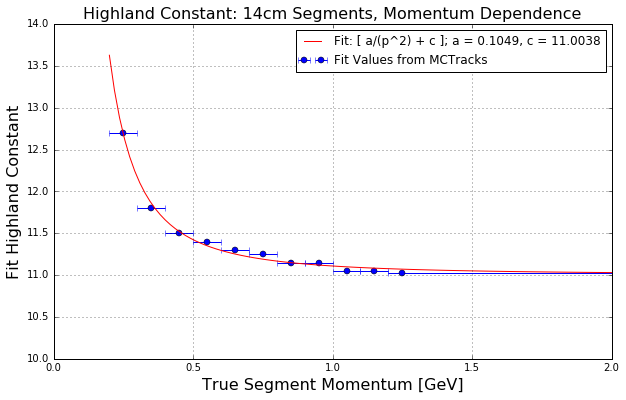
\includegraphics[width=100mm]{Figures/highland_constant_optimization_momentumdependent.png}
\end{center}
\caption{\textit{Fitted Highland constant as a function of true segment momentum for 14 cm segments of {\sc MCTracks}. Blue x- error bars indicate true momentum bin width with data points drawn at the center of each bin, except for the highest momentum bin which includes the segment momentum tail that extends beyond the limit of the plot, up to 6 GeV. Shown in red is a fit to these data points with functional form $\frac{a}{p^2} + c$, with converged values for floating constants $a$ and $c$ shown in the legend.}}
\label{retune_highland_fig3}
\end{figure}

Note that the highest momentum point in Figure \ref{retune_highland_fig3} represents a bin which extends from 1.10 GeV to 6 GeV, capturing the entire high momentum ($\beta = 1$) tail of the true {\sc MCTrack} segment momentum distribution. It can be seen that the fitted value asymptotically approaches a constant at higher momentum (where $\beta = 1$) of about 11.0. The value increases in the momentum region where $\beta < 1$. Shown in red is a fit to these data points with functional form $\frac{a}{p^2} + c$, with converged values for floating constants $a$ and $c$ shown in the legend. This functional form was chosen because it fit the data well, and asymptotically approaches a constant value when $\beta$ approaches 1. The fitted values for $a$ and $c$ are 0.1049 and 11.0038 respectively. This function will henceforth be referred to as $\kappa(p)$:
\begin{equation}
\kappa(p) = \frac{0.1049}{p^2} + 11.0038
\end{equation}\label{kappa_equation}

In this analysis, $\kappa(p)$ is used as a replacement for the 13.6 constant in the Highland formula. Note that with 14 cm segments, the smallest segment momentum the algorithm plugs into Equation \ref{kappa_equation} corresponds to the left-most value of the fit drawn, a Highland constant of about 13.7, so the rapid increase of $\kappa(p)$ for small values of $p$ is not an issue. The effect of replacing 13.6 with $\kappa(p)$ in the Highland equation is to reduce a systematic bias that was present in the algorithm, in which the algorithm overestimated the true momentum of muons. To visualize the Highland formula for 14 cm segments both before and after the $\kappa(p)$ replacement, see Figure \ref{retune_highland_fig4}. It is recommended that future LArTPC experiments use this parameterization of the Highland formula, or at the very least conduct their own studies fit for the 13.6 constant in the Highland formula, which clearly is not the correct value for liquid argon specifically.\\

\begin{figure}[ht!]
\begin{center}
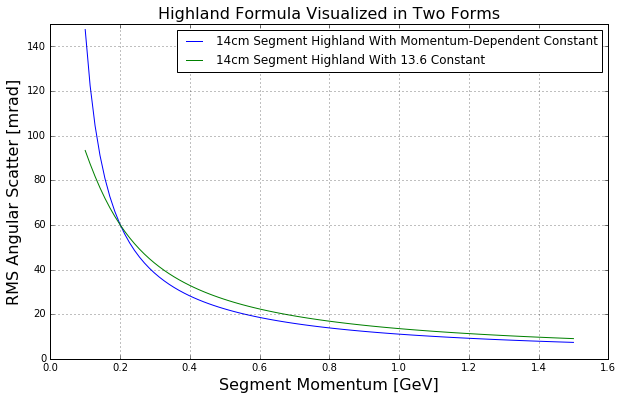
\includegraphics[width=100mm]{Figures/highland_formula_visualized_twoforms.png}
\end{center}
\caption{\textit{The Highland scattering RMS $\sigma_o$ for 14 cm segment lengths and 0 detector-inherent angular resolution as a function of true momentum before and after retuning. In green is shown Equation \ref{highland_simplified} (using 13.6 constant) and in blue is the same equation replacing 13.6 with $\kappa(p)$.}}
\label{retune_highland_fig4}
\end{figure}



The form of the Highland equation used in this analysis is therefore given by Equation \ref{modified_highland_eqtn}, with $\kappa(p)$ given by Equation \ref{kappa_equation}, noting that with segmentation length $\ell = X_0 = 14 cm$ the formula simplifies greatly. For the sake of readability, Equation \ref{modified_highland_eqtn} is rewritten here:
\begin{equation}
\sigma_{o}^{RMS} = \sqrt{ (\sigma_o)^2 + (\sigma_o^{res})^2} = \sqrt{ (\frac{\kappa(p)}{p\beta c}z\sqrt{\frac{\ell}{X_0}}\Big[1+0.0038\text{ln}\Big(\frac{\ell}{X_0}\Big)\Big])^2 + (\sigma_o^{res})^2 }
\end{equation}

